\documentclass[border=3pt,tikz]{standalone}
\usepackage[utf8]{vietnam}
\usetikzlibrary{calc,angles,intersections,shapes.geometric,arrows,decorations.markings,arrows.meta,patterns.meta,patterns}
\usepackage{tikz-3dplot,pgfplots}
\pgfplotsset{compat=1.15}
\usepgfplotslibrary{polar}
\usepackage{amsmath}
\begin{document}
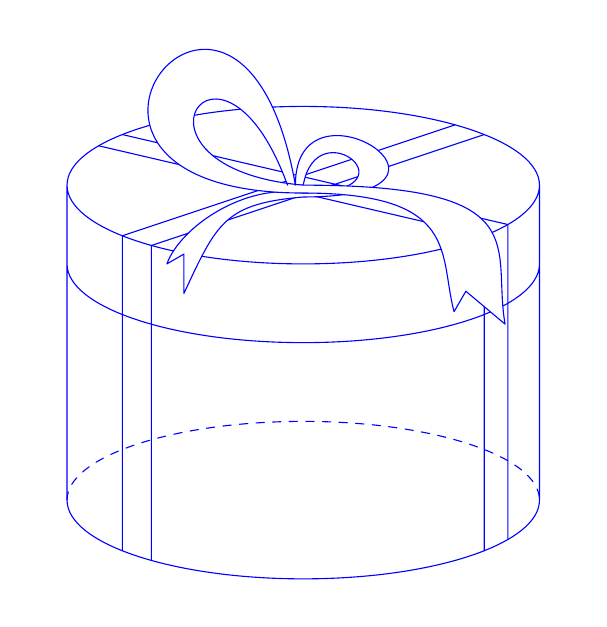
\begin{tikzpicture}[line join=round,line cap=round,blue]
	\def\h{4} %Chiều cao
	\def\a{3} %Chiều rộng
	\xdef\b{\a/3}
	\foreach \x [count=\i] in {40,50,140,150,220,230,320,330}{\path (\a,0) arc (0:\x:{\a} and {\b}) coordinate (A\i);}
	\clip (-\a-.5,\b+1) rectangle (\a+.5,-\h-\b-.25);
	\draw[dashed] (-\a,-\h) arc (180:0:{\a} and {\b});
	\draw
	(-\a,0)--(-\a,-\h) arc(180:360:{\a} and {\b})--(\a,0)
	(0,0) ellipse ({\a} and {\b})
	(-\a,-\h/4) arc (180:360:{\a} and {\b});
	;
	\draw
	(A1)--(A6)--++(-90:\h)
	(A2)--(A5)--++(-90:\h)
	(A3)--(A8)--++(-90:\h)
	(A4)--(A7)--++(-90:\h)
	;
	\draw[fill=white]
	(0,0) ..controls +(80:1) and +(0:1.5).. (-90:.1)
	..controls +(170:.75) and +(70:.5) ..(-150:2)--++(30:.25)--++(-90:.5)
	..controls +(65:1) and +(185:1)..(-90:.15)
	..controls +(0:2.5) and +(90:1.5) .. (180:.1)--cycle
	;
	\draw[fill=white]
	(180:.1) ..controls +(100:4) and +(180:4)..(-90:.1)
	..controls +(0:2) and +(105:.75) ..(-40:2.5)--++(60:.3)--++(-40:.65)
	..controls +(100:1) and +(0:3)..(0:0)
	..controls +(175:2.5) and +(110:2.5) ..(180:.2)
	;
\end{tikzpicture}
\end{document}